\section{Experiments}
\label{sec:experiments}

We report unconditional generation on MOSES in the main text and on QM9 in
Appendix~\ref{app:qm9-uncond}, conditional generation under property targets (logP, logS, QED, TPSA), and
geodesic comparisons in the learned space. By convention, on QM9 we report novelty separately from
$V.U.$: the dataset is small and novelty is often far from 1.0, so we include a dedicated novelty
column to show it is comparable and to avoid biasing \gls*{fcd} there.
We report validity (RDKit-sanitized non-empty SMILES), uniqueness (distinct SMILES among valid),
novelty (unique valid molecules not in the training split), and $V.U.N.$ for the fraction satisfying
all three. We also report \gls*{fcd}, a ChemNet feature-space distance between generated and MOSES
molecules (lower is better). We consider two initialization regimes. \textbf{Noise Initialization}
(standard for diffusion models) starts from easy-to-sample noise; the main challenge is to reach
chemically valid molecules, while novelty is often already high. \textbf{Data Initialization}
(available to energy-based models) starts from molecules drawn from the training dataset; the main
challenge is to make non-trivial edits that increase novelty while preserving chemical validity.
In practice, Noise Initialization uses \textbf{uniform noise} (node count from the empirical
histogram, node/edge types uniform) or \textbf{marginal noise} (node count from the empirical
histogram, node/edge types from empirical marginals), while Data Initialization uses \textbf{training
data} samples; sampling can be run with diffusion/CTMC dynamics or MCMC.
MOSES is a large-scale molecular dataset (about 1.5M molecules), while QM9 is a smaller benchmark
focused on low-mass molecules. We use MOSES to stress-test sample quality at scale and QM9 as a
compact setting for comparison.
%
A concise conceptual summary of the baselines used in our experiments is provided in
Appendix~\ref{app:baselines}, and the experimental setup is detailed in Appendix~\ref{app:exp-setup}.

\subsection*{Unconditional generation}
\paragraph{MOSES: Baselines vs.\ GEM.}
Table~\ref{tab:uncond-moses} reports unconditional metrics on MOSES; QM9 results are in
Appendix~\ref{app:qm9-uncond} (Table~\ref{tab:uncond-qm9}).
Figure~\ref{fig:moses-energy-and-metrics} reports annealed-proposal metrics on MOSES. Across both
Noise Initialization and Data Initialization, GEM improves V.U.N.\ and \gls*{fcd}.
Validity, novelty, and uniqueness can be
improved post-hoc via rejection sampling, so diffusion baselines already reach strong V.U.N., but
\gls*{fcd} is less amenable to such correction; we see a clear gap on MOSES. The step curves in
Figure~\ref{fig:moses-vun-steps} show rapid early gains with diminishing returns as steps increase,
and Figure~\ref{fig:moses-energy-and-metrics} highlights the distinct trajectories under Noise vs.\
Data Initialization.
\begin{table}[h]
\centering
\small
\textbf{MOSES} ($\sim$1.5M molecules)\\[2pt]
\begin{tabular}{lcc}
\toprule
Method & V.U.N. $\uparrow$ & \gls*{fcd} $\downarrow$ \\
\midrule
Training samples (MOSES) & 0.0 & 0.09 \\
\midrule
\multicolumn{3}{l}{\textit{Noise Initialization}} \\
\midrule
GraphEBM$^*$~\citep{liu2021graphebm} & 8.12 & 9.83 \\
VFM$^*$~\citep{eijkelboom2024vfm} & 81.39 & 2.71 \\
DeFoG$^*$~\citep{qinmadeira2024defog} & 82.21 & 1.95 \\
\textbf{GEM (Ours)} & \textbf{85.61} & \textbf{1.50} \\
\midrule
\multicolumn{3}{l}{\textit{Data Initialization}} \\
\midrule
GraphEBM$^*$~\citep{liu2021graphebm} & 32.16 & 7.31 \\
\textbf{GEM (Ours)} & \textbf{89.81} & \textbf{0.76} \\
\bottomrule
\end{tabular}
\caption{\footnotesize \textbf{Unconditional Generation.} MOSES results grouped by initialization.
$V.U.N.$ is the valid-unique-novel fraction (higher is better); \gls*{fcd} measures the distance
between generated and MOSES molecules in ChemNet feature space (lower is better). $^*$ reproduced
with the same backbone as DeFoG~\citep{qinmadeira2024defog}; EBMs use a small energy head. Architecture
details are in Appendix~\ref{app:perm-invariance}. 25k generations. Budget of 1000 inference steps.}
\label{tab:uncond-moses}
\end{table}

A schematic of MCMC evolution for GEM on QM9 and MOSES is shown in Appendix~\ref{app:sampling}
(Figure~\ref{fig:appendix-mcmc-traj}).

\begin{figure}[h]
\centering
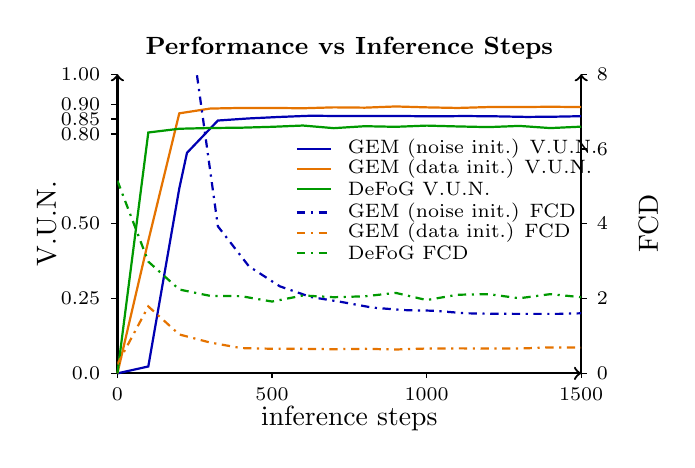
\begin{tikzpicture}[scale=0.95]
  \draw[->, thick] (0,0) -- (6.2,0) node[midway, below=8pt] {inference steps};
  \draw[->, thick] (0,0) -- (0,4.0);
  \node[rotate=90] at (-0.95,2.0) {V.U.N.};
  \draw[->, thick] (6.2,0) -- (6.2,4.0);
  \node[rotate=90] at (7.1,2.0) {FCD};

  % Title
  \node[font=\small\bfseries] at (3.1,4.35) {Performance vs Inference Steps};

  % Axes ticks
  \foreach \x/\lab in {0/0,2.067/500,4.133/1000,6.200/1500} {
    \draw (\x,0) -- (\x,-0.06);
    \node[below, font=\scriptsize] at (\x,-0.06) {\lab};
  }
  \foreach \y/\lab in {0/0.0,1.0/0.25,2.0/0.50,3.2/0.80,3.4/0.85,3.6/0.90,4.0/1.00} {
    \draw (0,\y) -- (-0.08,\y);
    \node[left, font=\scriptsize] at (-0.1,\y) {\lab};
  }
  \foreach \y/\lab in {0/0,1.0/2,2.0/4,3.0/6,4.0/8} {
    \draw (6.2,\y) -- (6.28,\y);
    \node[right, font=\scriptsize] at (6.28,\y) {\lab};
  }
  % Noise initialization (warmup + DLangevin)
  \draw[blue!70!black, thick] plot coordinates {
    (0.000,0.000) (0.413,0.092) (0.827,2.472) (0.930,2.948) (1.343,3.380)
    (1.757,3.408) (2.170,3.428) (2.583,3.444) (2.997,3.440) (3.410,3.440)
    (3.823,3.440) (4.237,3.436) (4.650,3.440) (5.063,3.436) (5.477,3.428)
    (5.890,3.432) (6.200,3.438)
  };

  % Data initialization (annealed)
  \draw[orange!90!black, thick] plot coordinates {
    (0.000,0.000) (0.413,1.772) (0.827,3.476) (1.240,3.540) (1.653,3.548)
    (2.067,3.548) (2.480,3.544) (2.893,3.556) (3.307,3.552) (3.720,3.568)
    (4.133,3.556) (4.547,3.548) (4.960,3.560) (5.373,3.560) (5.787,3.564)
    (6.200,3.560)
  };

  % DeFoG
  \draw[green!60!black, thick] plot coordinates {
    (0.000,0.000) (0.413,3.220) (0.827,3.270) (1.240,3.280) (1.653,3.284)
    (2.067,3.296) (2.480,3.313) (2.893,3.278) (3.307,3.304) (3.720,3.296)
    (4.133,3.312) (4.547,3.301) (4.960,3.292) (5.373,3.308) (5.787,3.279)
    (6.200,3.298)
  };

  % FCD (right axis)
  \begin{scope}
    \clip (0,0) rectangle (6.2,4.0);
    \draw[blue!70!black, thick, dash dot] plot coordinates {
      (0.413,8.184) (0.827,4.961) (0.930,4.952) (1.343,1.966) (1.757,1.432)
      (2.170,1.164) (2.583,1.021) (2.997,0.954) (3.410,0.879) (3.823,0.846)
      (4.237,0.837) (4.650,0.803) (5.063,0.796) (5.477,0.795) (5.890,0.795)
      (6.200,0.803)
    };
    \draw[orange!90!black, thick, dash dot] plot coordinates {
      (0.000,0.122) (0.413,0.895) (0.827,0.520) (1.240,0.412) (1.653,0.338)
      (2.067,0.329) (2.480,0.328) (2.893,0.323) (3.307,0.328) (3.720,0.319)
      (4.133,0.332) (4.547,0.334) (4.960,0.333) (5.373,0.332) (5.787,0.347)
      (6.200,0.344)
    };
    \draw[green!60!black, thick, dash dot] plot coordinates {
      (0.000,2.575) (0.413,1.494) (0.827,1.121) (1.240,1.036) (1.653,1.032)
      (2.067,0.960) (2.480,1.041) (2.893,1.018) (3.307,1.030) (3.720,1.076)
      (4.133,0.980) (4.547,1.051) (4.960,1.059) (5.373,1.004) (5.787,1.059)
      (6.200,1.018)
    };
  \end{scope}

  % Legend
  \begin{scope}[shift={(2.25,1.35)}]
    \draw[blue!70!black, thick] (0.15,1.65) -- (0.6,1.65);
    \node[anchor=west, font=\scriptsize] at (0.7,1.65) {GEM (noise init.) V.U.N.};
    \draw[orange!90!black, thick] (0.15,1.38) -- (0.6,1.38);
    \node[anchor=west, font=\scriptsize] at (0.7,1.38) {GEM (data init.) V.U.N.};
    \draw[green!60!black, thick] (0.15,1.11) -- (0.6,1.11);
    \node[anchor=west, font=\scriptsize] at (0.7,1.11) {DeFoG V.U.N.};
    \draw[blue!70!black, thick, dash dot] (0.15,0.80) -- (0.6,0.80);
    \node[anchor=west, font=\scriptsize] at (0.7,0.80) {GEM (noise init.) FCD};
    \draw[orange!90!black, thick, dash dot] (0.15,0.53) -- (0.6,0.53);
    \node[anchor=west, font=\scriptsize] at (0.7,0.53) {GEM (data init.) FCD};
    \draw[green!60!black, thick, dash dot] (0.15,0.26) -- (0.6,0.26);
    \node[anchor=west, font=\scriptsize] at (0.7,0.26) {DeFoG FCD};
  \end{scope}
\end{tikzpicture}
\caption{\footnotesize \textbf{V.U.N. and FCD vs Steps.} V.U.N. (higher is better) and FCD (lower is better) versus inference steps on MOSES for GEM noise initialization (uniform) with greedy warmup proposal, GEM data initialization with annealed proposal, and DeFoG (marginal noise).}
\label{fig:moses-vun-steps}
\end{figure}











\paragraph{QM9.}
QM9 unconditional metrics are reported in Appendix~\ref{app:qm9-uncond}
(Table~\ref{tab:uncond-qm9}).

\subsection*{Conditional generation}
We evaluate conditional generation under molecular property constraints (e.g., logP, QED).
We train a property regressor \(f_\phi\) (GraphTransformer) for differentiable guidance and define a
conditioned energy \(V_\theta^{\mathrm{cond}}(x)=V_\theta(x)+\lambda_{\mathrm{prop}}\|f_\phi(x)-y^\star\|^2\),
then run the same proposal kernel $q_\theta(x\!\to\!y)$ using \(-\nabla_x V_\theta^{\mathrm{cond}}(x)\),
with the Metropolis--Hastings acceptance ratio modified accordingly. For fairness, all methods use
noise-conditioned regressors; GEM also admits clean regressors, so we report a clean-regressor
ablation in Appendix~\ref{app:regressor-noise} (Figure~\ref{fig:regressor-noise},
Table~\ref{tab:regressor-ablations}). Noise-conditioned regressors are more reliable on noisy or
invalid graphs (and we often must traverse such regions to move between modes), so they provide more
stable guidance. Baselines follow their standard marginal-noise regressors, while GEM uses
uniform-noise conditioning (our training noise), with all other settings matched. We choose targets
(e.g., logS $\ge$ -2.25, logP $\le$ 1.5, QED $\ge$ 0.9, TPSA $\le$ 50) so that unconditional MOSES
samples satisfy the constraint at roughly a 20\% rate, yielding comparable difficulty across
properties.
Table~\ref{tab:moses-conditional} reports single-property conditioning results, and
Appendix~\ref{app:baselines} summarizes joint constraints (Table~\ref{tab:moses-conditional-joint}).
GEM maintains strong validity, uniqueness, and novelty while improving constraint satisfaction
relative to baselines.
GEM draws a candidate pool of size $N_{\mathrm{select}}$ from the training set, ranks by the
precomputed property values, and initializes the $B$ inference chains with the top-$B$ molecules
that satisfy the condition; this takes virtually no time because the training-set properties are
cached.

\begin{table*}[t]
\centering
\small
\textbf{MOSES} ($\sim$1.5M molecules)\\[2pt]
\begingroup
\setlength{\tabcolsep}{3pt}
\begin{tabular}{lcc cc cc cc}
\toprule
Method
& \multicolumn{2}{c}{Condition: logS $\ge$ -2.25}
& \multicolumn{2}{c}{Condition: \acrshort{qed} $\ge$ 0.9}
& \multicolumn{2}{c}{Condition: \acrshort{tpsa} $\le$ 50}
& \multicolumn{2}{c}{Condition: logP $\le$ 1.5} \\
\cmidrule(lr){2-3} \cmidrule(lr){4-5} \cmidrule(lr){6-7} \cmidrule(lr){8-9}
& \glsentryshort{cvun} $\uparrow$ & \glsentryshort{cvu} $\uparrow$
& \glsentryshort{cvun} $\uparrow$ & \glsentryshort{cvu} $\uparrow$
& \glsentryshort{cvun} $\uparrow$ & \glsentryshort{cvu} $\uparrow$
& \glsentryshort{cvun} $\uparrow$ & \glsentryshort{cvu} $\uparrow$ \\
\midrule
Training samples (MOSES) & 0 & 0.24 & 0 & 0.16 & 0 & 0.21 & 0 & 0.15 \\
\midrule
\multicolumn{9}{l}{\textit{Noise Initialization}} \\
\midrule
G-\gls{vfm}$^*$~\citep{eijkelboom2025controlledvfm} & 0.72 & 0.75 & 0.26 & 0.28 & 0.72 & 0.80 & 0.70 & 0.74 \\
DeFoG$^*$~\citep{qinmadeira2024defog} & 0.74 & 0.79 & 0.26 & 0.31 & 0.77 & \textbf{0.82} & 0.78 & 0.82 \\
\textbf{\gls{gem} (Ours)} & \textbf{0.80} & \textbf{0.81} & \textbf{0.40} & \textbf{0.40} & \textbf{0.80} & 0.81 & \textbf{0.85} & \textbf{0.85} \\
\bottomrule
\end{tabular}
\endgroup
\vspace{0.15cm}
\caption{\footnotesize \textbf{Property Conditioning.} MOSES conditional generation under property constraints. \gls{cvun} is the fraction meeting the condition and valid, unique, novel simultaneously; \gls{cvu} is the fraction meeting the condition and valid, unique. All entries are percentages. $C$, $V$, $U$, and $N$ denote condition satisfaction, validity, uniqueness, and novelty, respectively. 1k inference steps. Evaluated on 5k samples.$^*$ reproduced, same architecture (other than a small energy-head for \gls{gem} \cref{app:perm-invariance}).}
\label{tab:moses-conditional}
\vspace{-5pt}
\end{table*}



\subsection*{Geodesic analysis}
We compute geodesics between molecules and compare against a linear interpolation baseline.
All alignments are within fixed node counts, using node-matching to define couplings between pairs.
We sample 1000 molecules, form same-size pairs, and for each pair construct (i) an energy-weighted
geodesic and (ii) a linear interpolation along the coupling. From the continuous path we obtain
discrete graphs via categorical sampling, then compute the average validity along each path.
We plot average validity versus the endpoint distance induced by the matching cost
$c_{\mathrm{FGW}}$ (node-matching, Appendix~\ref{app:matching}), comparing geodesic vs.\ linear;
see Figure~\ref{fig:geodesic-validity}. Qualitative paths are shown in
Figure~\ref{fig:mol-trajectories}.
We report the length ratio $L_{\mathrm{geo}}/L_{\mathrm{lin}}$ and the correlation between energy and
validity along the path; energy-weighted geodesics consistently preserve validity and shorten paths
relative to cost-only geodesics, confirming that the learned energy captures chemically meaningful
geometry.

\begin{figure*}[htbp]
\centering
\begin{tikzpicture}[scale=1.15]
  % Layout constants
  \def\boxsize{2.4}
  \def\gap{2.5}
  \def\rowgap{2.3}
  \def\arrowlen{0.3}

  % Row 1 (GEM, skip duplicate C)
  \foreach \fname [count=\i from 0] in {
      figures/interpolation/gem_00,
      figures/interpolation/gem_01,
      figures/interpolation/gem_03,
      figures/interpolation/gem_04,
      figures/interpolation/gem_05,
      figures/interpolation/gem_06} {
    \node[inner sep=0pt] at (\i*\gap+0.5*\boxsize,0.5*\boxsize)
      {\includesvg[width=\boxsize cm]{\fname}};
    \node[anchor=north west, font=\scriptsize\bfseries] at (\i*\gap+0.05*\boxsize,0.98*\boxsize)
      {\ifnum\i=0 initial\else\ifnum\i=5 final\else\relax\fi\fi};
  }
  \foreach \i in {0,1,2,3,4} {
    \draw[->, line width=0.4pt, opacity=0.3]
      ({\i*\gap + 0.5*(\gap+\boxsize) - 0.5*\arrowlen}, {0.5*\boxsize})
      -- ({\i*\gap + 0.5*(\gap+\boxsize) + 0.5*\arrowlen}, {0.5*\boxsize});
  }

  % Row 2 (linear, skip duplicate C)
  \foreach \fname [count=\i from 0] in {
      figures/interpolation/linear_00,
      figures/interpolation/linear_01,
      figures/interpolation/linear_03,
      figures/interpolation/linear_04,
      figures/interpolation/linear_05,
      figures/interpolation/linear_06} {
    \node[inner sep=0pt] at (\i*\gap+0.5*\boxsize,-\rowgap+0.5*\boxsize)
      {\includesvg[width=\boxsize cm]{\fname}};
    \node[anchor=north west, font=\scriptsize\bfseries] at (\i*\gap+0.05*\boxsize,-\rowgap+0.98*\boxsize)
      {\ifnum\i=0 initial\else\ifnum\i=5 final\else\relax\fi\fi};
  }
  \foreach \i in {0,1,2,3,4} {
    \draw[->, line width=0.4pt, opacity=0.3]
      ({\i*\gap + 0.5*(\gap+\boxsize) - 0.5*\arrowlen}, {-\rowgap+0.5*\boxsize})
      -- ({\i*\gap + 0.5*(\gap+\boxsize) + 0.5*\arrowlen}, {-\rowgap+0.5*\boxsize});
  }

  % Row labels (above rows)
  \node[anchor=west, font=\small\bfseries] at (0,\boxsize+0.30) {GEM energy-weighted geodesic:};
  \node[anchor=west, font=\small\bfseries] at (0,-\rowgap+\boxsize+0.30) {Cost-only geodesic:};
\end{tikzpicture}
\caption{\footnotesize \textbf{GEM Energy-Weighted vs Cost-Only Geodesics.} Molecule trajectories along continuous geodesic paths for MOSES. Top row: GEM energy-weighted geodesic; bottom row: cost-only geodesic. Boxes indicate samples along the continuous path.}
\label{fig:mol-trajectories}
\end{figure*}








We implement the geodesic path as a spline (Bezier) interpolation over node/edge logits in the
probability simplex, then sample discrete graphs along evenly spaced points on the path. The linear
baseline uses the same endpoints and sampling protocol. Appendix~\ref{app:geodesic-details} provides
the implementation details.
 
In the embedding space we consider paths $\hat{\gamma}(t)$ and use the local geometry induced by
\eqref{eq:loc-cost}. Define
\begin{equation}
\|\dot{\hat{\gamma}}(t)\|_{\mathrm{loc}}^2
=\lambda_X\sum_{i\in\mathcal{V}}\|\dot{\hat{\gamma}}_i(t)\|^2
+\lambda_E\sum_{i<j}\|\dot{\hat{\gamma}}_{ij}(t)\|^2,
\end{equation}
and the energy-weighted length
\begin{equation}
L_\theta(\gamma)=\int_0^1 \exp\!\big(\beta V_\theta(\hat{\gamma}(t))\big)\,
\|\dot{\hat{\gamma}}(t)\|_{\mathrm{loc}}\,\mathrm{d}t.
\end{equation}
We optimize the geodesic objective
\begin{equation}
\mathcal{J}_{\mathrm{geo}}(\gamma)
=
L_\theta(\gamma)
\;+\lambda_{ME}\int_0^1 V_\theta(\hat{\gamma}(t))\,\mathrm{d}t,
\end{equation}
Additional details are in Appendix~\ref{app:geodesic-details}.

\begin{figure}[H]
\centering
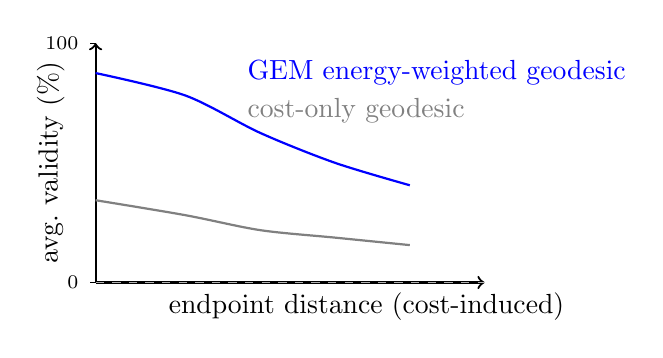
\begin{tikzpicture}[scale=0.95]
  \draw[->, thick] (0,0) -- (5.2,0) node[below, xshift=-1.5cm] {endpoint distance (cost-induced)};
  \draw[->, thick] (0,0) -- (0,3.2);
  \node[rotate=90] at (-0.6,1.6) {avg.\ validity (\%)};

  \draw (0,0) -- (-0.08,0);
  \node[left, font=\scriptsize] at (-0.1,0) {0};
  \draw (0,3.2) -- (-0.08,3.2);
  \node[left, font=\scriptsize] at (-0.1,3.2) {100};

  \draw[gray!60, dashed] (0,0) -- (5.2,0);

  \draw[thick, blue] plot[smooth] coordinates {(0.0,2.8) (1.2,2.5) (2.2,2.0) (3.2,1.6) (4.2,1.3)};
  \draw[thick, gray] plot[smooth] coordinates {(0.0,1.1) (1.2,0.9) (2.2,0.7) (3.2,0.6) (4.2,0.5)};

  \node[blue, anchor=west] at (1.9,2.8) {GEM energy-weighted geodesic};
  \node[gray, anchor=west] at (1.9,2.3) {cost-only geodesic};
\end{tikzpicture}
\caption{\footnotesize \textbf{Validity Along Geodesics.} Expected average validity vs.\ endpoint distance (cost-induced) for GEM energy-weighted versus cost-only geodesics.}
\label{fig:geodesic-validity}
\end{figure}
